\chapter{Algorytm - poszczególne składowe oraz przykłady zastosowania}
\label{cha:AlgorytmPraktyka}

\newpage
\section{Przejścia dla pieszych}
\label{sec:pedestrialCrossing}
\subsection{Przyporządkowywanie przejść dla pieszych do poszczególnych dróg}

Bardzo ważnym czynnikiem doboru prędkości jest obecność przejść dla pieszych. Te z sygnalizacją świetlną nie stanowią problemu, ponieważ ruch pieszych poruszających się na nich jest ograniczony tylko do sytuacji, gdy sygnalizacja świeci się na zielono. W przypadku przejść bez sygnalizacji, sprawa się komplikuje, ponieważ kierowca jest zobowiązany do zachowania szczególnej ostrożności i zmiejszenia prędkości od 30 km/h.

Do przyporządkowania przejść dla pieszych, do poszczególnych dróg, posłużyłem się wzorem \ref{eq:distancePointLineal} na odległość punktu od prostej, przedstawionym w sekcji \ref{sec:ObiektyPunktDrogi}.


Rezultatem wdrożenia powyższego wzoru do programu, są:
\begin{itemize}
\item na niebiesko zaznaczone drogi, na których znajdują się przejścia dla pieszych
\item znakiem ''D-6'' zostały oznaczone przejścia dla pieszych
\end{itemize}
Wynik został przedstawiony na Rys. \ref{sec:PrzejscieDrogi}:

\begin{figure}[h]
\caption{Drogi na których znajdują się przejścia dla pieszych.}
\label{sec:PrzejscieDrogi}
\centering
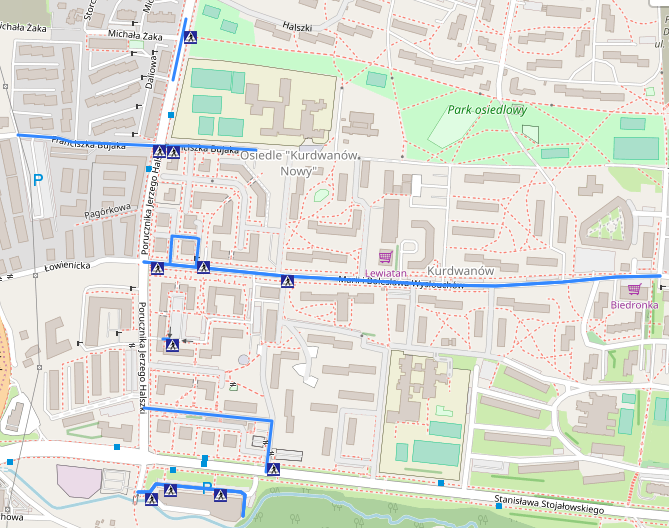
\includegraphics[width=0.9\textwidth]{PrzejscieDrogi}
\end{figure}

Dzięki tak zobrazowanej sytuacji, można ocenić skuteczność algorytmu przyporządkowującego przejścia dla pieszych do określonych dróg.

\subsection{Wyznaczanie prędkości i umieszczanie jej w odpowiednim miejscu na mapie}

Bezpieczna prędkość w pobliżu nieoznakowanych przejść dla pieszych wynosi ok. 30 km/h. Zapewnia ona zarówno wystarczajacy czas reakcji, odpowiednio krótką drogę hamowania oraz zmiejsza ryzyko wystąpień potrąceń pieszych.

Algorytm umieszcza znaki ograniczenia prędkości:
\begin{itemize}
\item w przypadku gdy maksymalna prędkość na drodze jest mniejsza bądź równo 30 km/h, nie ma sensu wstawiać znaku
\item w odległości 50 m od przejścia, gdy maksymalna prędkość na drodze jest mniejsza bądź równa 60 km/h
\item w odległości 150 m od przejścia, gdy maksymalna prędkość przekracza 60 km/h
\item w przypadku, gdy przejście dla pieszych znajduje się w odległości mniejszej niż 50m lub 150m (w zależności od maksymalnej prędkości), znak zostanie umieszczony na początku drogi
\item w przypadku drogi jednokierunkowej, tylko przed przejściem
\item w przypadku drogi dwukierunkowej, zarówno przed, jak i za przejściem
\item bezpośrednio za przejściem zostanie ustawiony znak przywracającą poprzednie ograniczenie prędkości, za wyjątkiem sytuacji, gdy droga za przejściem dla pieszych jest krótsza niż 100m. W takim wypadku, nie ma sensu zmieniać prędkości.
\end{itemize}

\begin{figure}[h]
\caption{Ograniczenia prędkości przy przejściach dla pieszych.}
\label{sec:przejsciePredkosci}
\centering
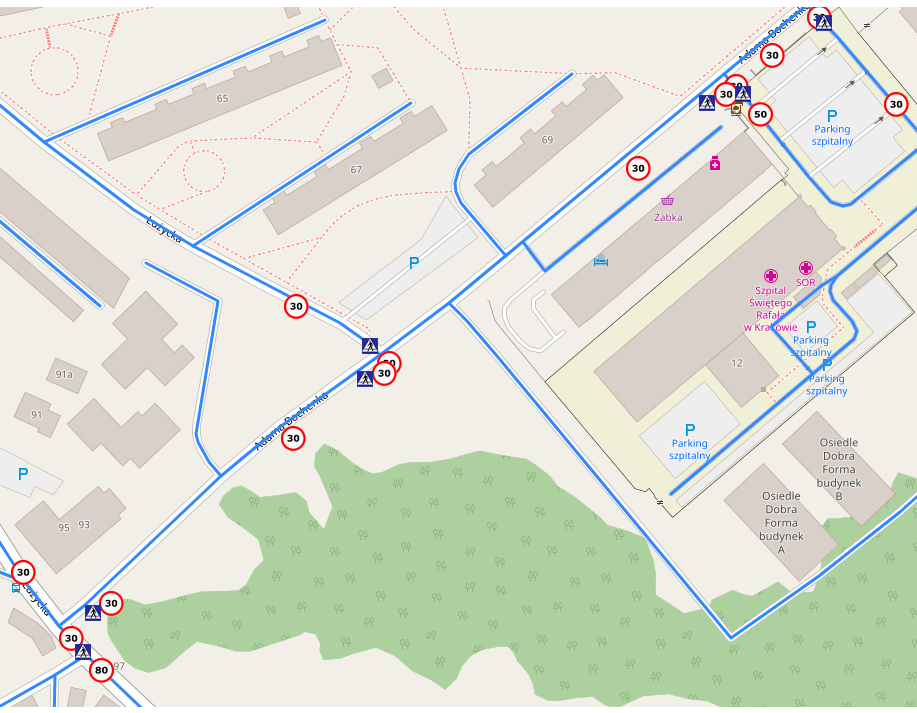
\includegraphics[width=0.7\textwidth]{pedestrian_speed}
\end{figure}

\newpage
\section{Typ nawierzchni}
\label{sec:surfaceType}

W celu zadbania o bezpieczeństwo osób, ale również o dobrą kondycję techniczną pojazdów poruszających się po drogach, niezbędne jest uwzględnienie typu nawierzchni. Nie można dopuścić do sytuacji, gdy na nawierzchni składającej się głównie że żwiru, znajdowało się znak ograniczenia prędkości o wysokiej wartości. Wtedy ulec awarii może zarówno zawieszenie, jak również pojazdy jadące przed nimi pojazdami. Aby zapoabiec tego typu problemom, podzieliłem typ nawierzchni na kilka rodzajów:

\begin{itemize}
\item kostka brukowa
\item żwir
\item drobny żwir
\item nieutwardzana
\item błotnista
\item płyty  betowowe
\item droga gruntowa
\item piasek
\item asfalt
\end{itemize}

Najbardziej problematyczna dla kierowów droga to taka, która pokryta jest żwirem, drobnym żwirem, składająca się z piasku lub jest błotnista. W takich przypadkach ograniczyłem prędkość do 10 km/h. Niewiele lepsza nawierzchnia to taka, która wyłożona jest zarówno kostką brukową oraz płytami betonowymi. Dla nich, odpowiednia prędkość wynosi 20 km/h. W przypadku drogi nieutwardzanej oraz gruntowej, ograniczenie prędkości wynosi 30 km/h. Dla asfaltu, ze względu na jego strukturę, ograniczenie prędkości praktycznie nie występuje.

Na Rys. \ref{sec:surfaceTypePhoto} zostały umieszczone ograniczenia prędkości dla dróg, których nawierzchnia pokryta jest materiałem innym niż asfalt. Dla celów demonstracyjnych, został on specjalnie pominięty, ponieważ więszkość dróg jest nim pokryta, przez co Rys. \ref{sec:surfaceTypePhoto} stałby się mało czytelny. Oczywiście ogólny algorytm uwzględnia asfalt.

\newpage
\begin{figure}[h]
\caption{Ograniczenia prędkości ze względu na rodzaj nawierzchni.}
\label{sec:surfaceTypePhoto}
\centering
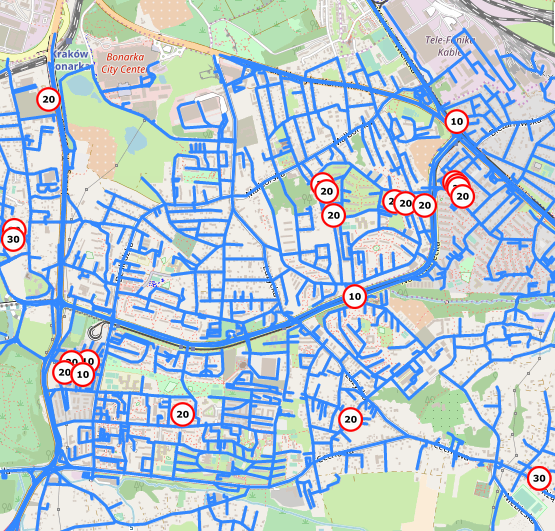
\includegraphics[width=0.9\textwidth]{surfaceType}
\end{figure}

\newpage
\section{Przejazdy kolejowe}
\subsection{Przyporządkowywanie przejazdów kolejowych do poszczególnych dróg}

Istotnych parametrem algorytmu wyznaczającego dopuszczalne prędkości jest obecność przejazdów kolejowych. Jak wiadomo, pociąg nie zatrzyma się w miejscu. Jego droga chamowania w głównej mierze zależy od masy oraz prędkości z jaką się porusza. Dla przykładu, pociąg towarowy o masie ok. 1800 ton, jadący z prędkością ok. 50 km/h, zatrzyma sie po około 500m. Dlatego ważne jest określenie prędkości, z jaką samochód moze się przemieszczać przed takim przejazdem.

Do przyporządkowania przejazdów kolejowych do poszczególnych dróg, wykorzystałem wzór \ref{eq:distancePointLineal} znajdujący się w rozdziale \ref{sec:pedestrialCrossing}


\begin{figure}[h]
\caption{Drogi na których znajdują się przejazdy kolejowe.}
\label{sec:PrzejazdyKolejowe}
\centering
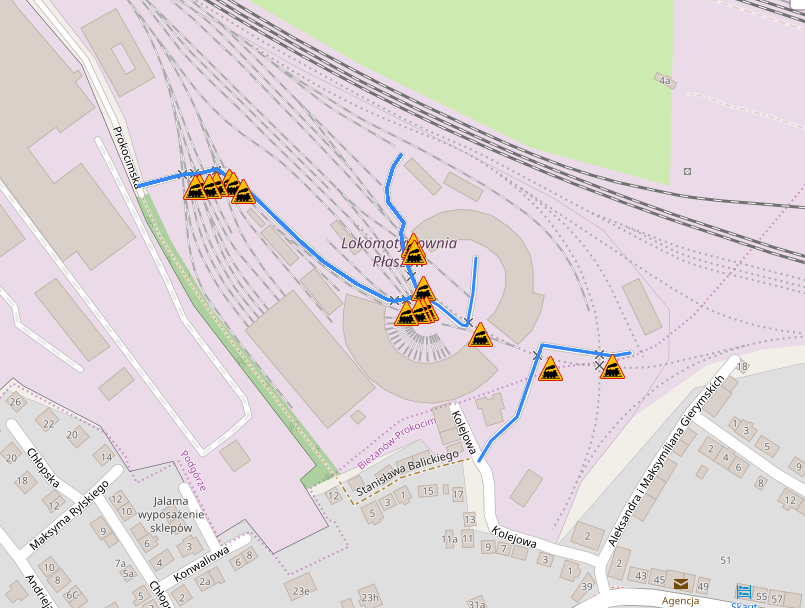
\includegraphics[width=1.0\textwidth]{railCrossing}
\end{figure}

Rys. \ref{sec:PrzejazdyKolejowe} obrazuje wynik przypisania przejazdów kolejowych do poszczególnych dróg:
\begin{itemize}
\item kolorem niebieskim drogi, na ktorych znajdują przejazdy kolejowe
\item znakiem ''A-10'' zostały oznaczone przejazdy kolejowe, pobrane z OpenStreetMap
\end{itemize}

\newpage
\subsection{Wyznaczanie prędkości i umieszczanie jej w odpowiednim miejscu na mapie}

Podobnie jak miało to miejsce w rozdziale \ref{sec:pedestrialCrossing}, umiejscowienie znaków przed przejazdem będzie zależało od kilku czynników:
\begin{itemize}
\item w przypadku gdy maksymalna prędkość na drodze jest mniejsza bądź równo 30 km/h, nie ma sensu wstawiać znaku
\item na  drodze z ograniczeniem prędkości do 60 km/h, znak zostanie umieszczony 50m przed przejazdem kolejowym
\item w przypadku prędkości powyżej 60 km/h, znak zostanie umieszczony w odległości 150m przed przejazdem kolejowym
\item w przypadku drogi jednokierunkowej, tylko przed przejazdem kolejowym
\item w przypadku drogi dwukierunkowej, zarówno przed, jak i za przejazdem
\item bezpośrednio za przejazdem zostanie ustawiony znak przywracającą poprzednie ograniczenie prędkości, za wyjątkiem sytuacji, gdy droga za przejazdem kolejowym jest krótsza niż 100m. W takim wypadku, nie ma sensu zmieniać prędkości.
\end{itemize}

Rys. \ref{sec:PrzejazdyKolejowe1} obrazuje przejazd kolejowy znajdujący się na dwukierunkowej drodze, na której obowiązuje ograniczenie prędkości do 80 km/h. Dlatego znaki 30 km/h zostały umieszczone 150m przed przejazdem, a zaraz po nim znaki przywracające poprzednią prędkość 80 km/h. Znaki są po obu stronach, gdyż jest do droga dwukierunkowa

\begin{figure}[h]
\caption{Umiejscowienie znaków przed i za przejazdem kolejowym.}
\label{sec:PrzejazdyKolejowe1}
\centering
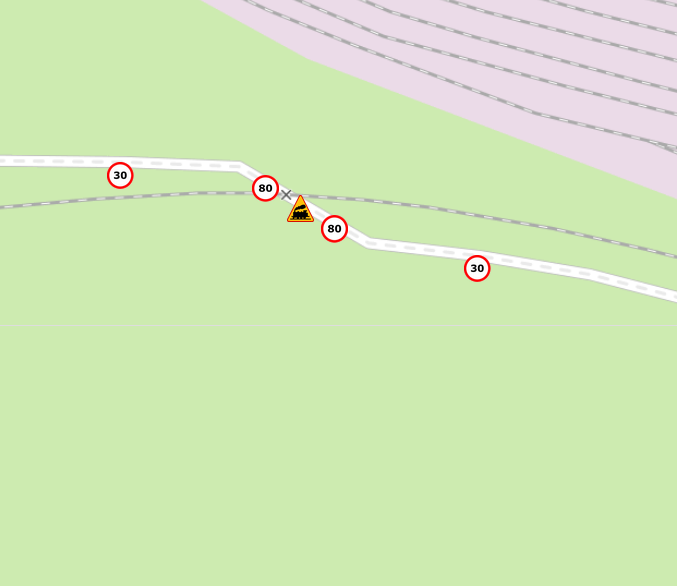
\includegraphics[width=0.6\textwidth]{streetBeforeRail}
\end{figure}


\newpage
\section{Sygnalizacja świetlna}
\subsection{Przyporządkowywanie sygnalizacji świetlnej do poszczególnych dróg}

Aby kierowca bez problemu mógł zdążyć zareagować na zmieniające się swiatło sygnalizacji świetlnej, niezbędne jest zredukowanie prędkości do odpowiedniej wartości. Ze względu na fakt iż sygnalizacja widoczna jest z relatywnie dużej odległości, prędkość przed nią zostanie ograniczona do ok. 50 km/h.


\begin{figure}[h]
\caption{Drogi na których znajduje się sygnalizacja świetlna.}
\label{sec:PrzejazdyKolejowe2}
\centering
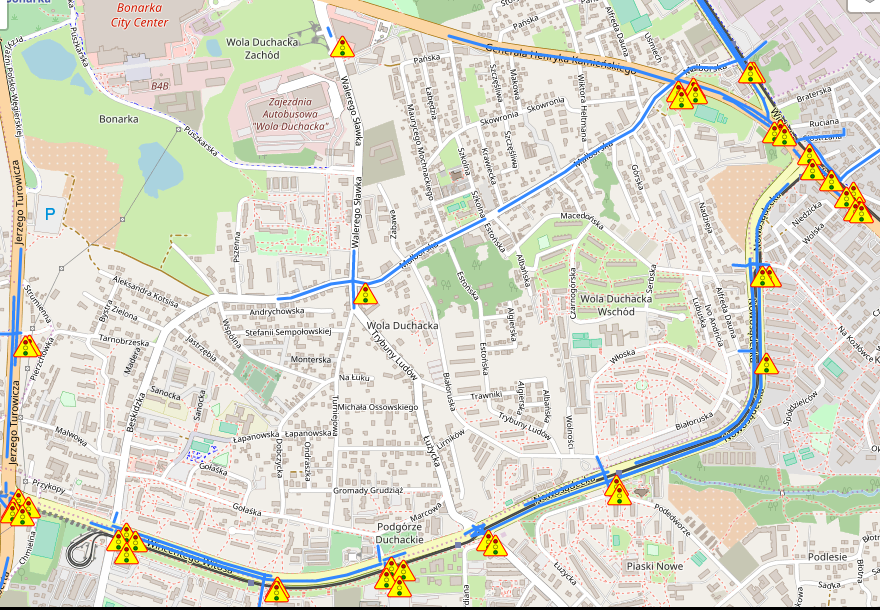
\includegraphics[width=1.1\textwidth]{traffic_sight}
\end{figure}

Rys. \ref{sec:PrzejazdyKolejowe2} ukazuje sposób działania algorytmu przypisującego do drogi sygnalizację świetlną. Zaznaczono na nim:
\begin{itemize}
\item kolorem niebieskim drogi, na ktorych znajduje się sygnalizacja świetlna
\item znakiem ''A-29'' zostały oznaczone sygnalizacje świetlne, pobrane z OpenStreetMap
\end{itemize}

\newpage
\subsection{Wyznaczanie prędkości i umieszczanie jej w odpowiednim miejscu na mapie}

Algorytm umieszcza znaki ograniczenia prędkości w następujący spasób:
\begin{itemize}
\item w przypadku gdy maksymalna prędkość na drodze jest mniejsza bądź równo 50 km/h, nie ma sensu wstawiać znaku
\item 50m przed sygnalizacją na drodze z ograniczeniem prędkości do 60 km/h
\item 150m przed sygnalizacją na drodze z ograniczeniem prędkości powyżej 60 km/h
\item w przypadku drogi dwukierunkowej, zarówno przed, jak i za przejazdem
\end{itemize}


Rys. \ref{sec:znakiSwiatla} obrazuje fragment skrzyżowania na której znajduje się sygnalizacja świetlna. Ograniczenie prędkości na drogach wynosi od 70 do 80 km/h, dlatego algorytm umieścił znak ograniczenia prędkości do 50 km/h, 150m przed sygnalizacją oraz znak przywracający poprzednią prędkość zaraz za sygnalizacją.

\begin{figure}[h]
\caption{Ograniczenie predkości przed i za światłami drogowymi}
\label{sec:znakiSwiatla}
\centering
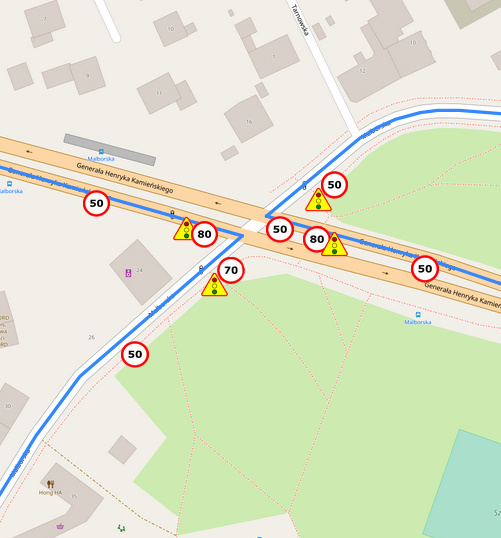
\includegraphics[width=0.8\textwidth]{speedBeforeSignals}
\end{figure}

\newpage
\section{Przystanki autobusowe i tramwajowe}
Kolejnymi obiektami, uwzględnionymi przez algorytm są przystanki autobusowe i tramwajowe. W ich pobliżu przeważnie znajduje się dość duża grupa ludzi w różnym przedziale wieku. Ponadto zdażają się sytuacje, że piesi wbiegają na drogę w celu zdążenia na komunikację miejską. Ze względu na takie zachowanie, algorytm ograniczy prędkość przy przystankach autobusowych do 30 km/h.

Na rys. \ref{sec:busStopBorder} zostały przedstawione przystanki autobusowe i tramwajowe. Wokół nich znajdują się powiększone o 5 metrów obszary pokrywający te obiekty.
\begin{figure}[h]
\caption{Ograniczenie predkości przed i za światłami drogowymi}
\label{sec:busStopBorder}
\centering
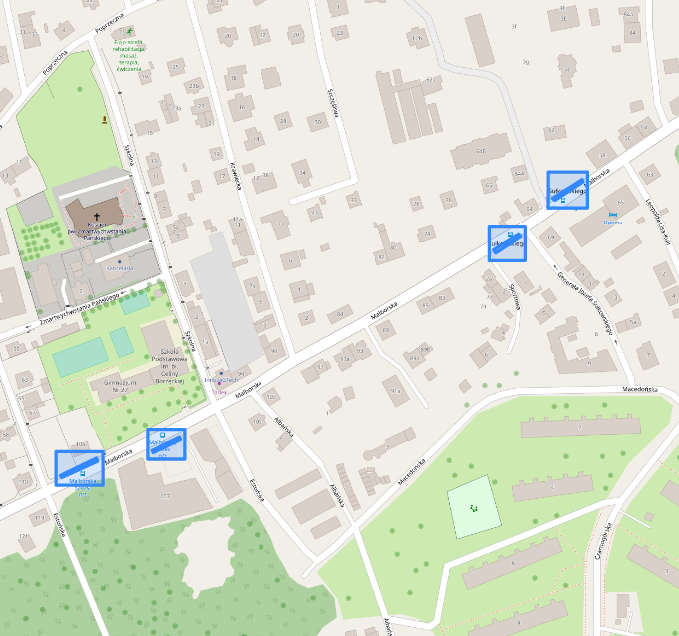
\includegraphics[width=0.9\textwidth]{busStopBorder}
\end{figure}


\newpage
\subsection{Wyznaczanie prędkości i umieszczanie jej w odpowiednim miejscu na mapie}

Najczęściej przystanki autobusowe i tramwajowe znajdują się na drogach o niezbyt wysokiej dopuszczalnej prędkości. W przypadku gdy dopuszczalna prędkość na drodze nie przekracza 30 km/h, nie ma sensu stawiać znak. W przypadku większej prędkości znak zostanie postawiony w odległości 20 metrów od powiększonego obszaru wokół przystanku, a znak przywracający poprzednią prędkość zaraz za nim. Opisana sytuacja została przedstawiona na rys. ...

\newpage
\section{Szkoły i miesca zabaw}


\newpage
\section{Sklepy i miejsca kultów religijnych}


\newpage
\section{Liczba pasów ruchu}

Maksymalna dozwolona prędkość jest zależna również od liczby pasów ruchu. Im jest ich więcej, tym większą prędkość można rozwijać. Dlatego algorytm zwiększa dopuszczalną prędkość o 10 km/h w przypadku gdy liczba pasów ruchu jest większa niż jeden. Na rys \ref{sec:laneNumber} zostały zaznaczone ulice, których liczba pasów ruchu wynosi przynajmniej 2, oraz prędkości nie uwzględniające pasów ruchu. 

\begin{figure}[h]
\caption{Prędkość przy nie uwgzględnieniu liczby pasów ruchu}
\label{sec:laneNumber}
\centering
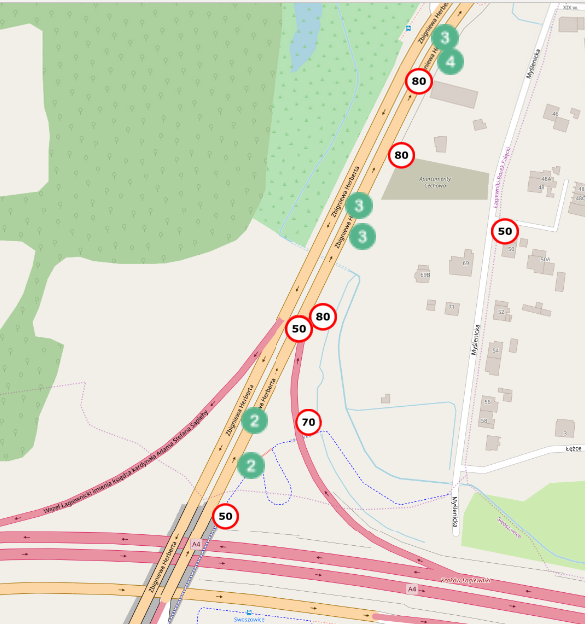
\includegraphics[width=0.9\textwidth]{laneNumber}
\end{figure}

\newpage
Na rys. \ref{sec:laneNumberAfter} zostały przedstawione prędkości już z uwzlędnioną liczbą pasów ruchu.
\begin{figure}[h]
\caption{Prędkość uwzględniająca liczbę pasów ruchu}
\label{sec:laneNumberAfter}
\centering
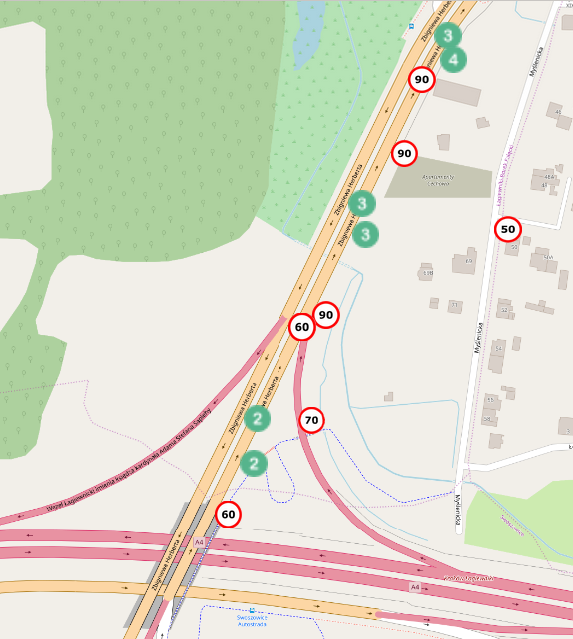
\includegraphics[width=0.9\textwidth]{laneNumberAfter}
\end{figure}

\newpage
\section{Rodzaj drogi}
Algorytm rozróżnia sześć podstawowych typów dróg, w skład których wchodzą:
\begin{itemize}
\item dojazdowe
\item lokalne
\item główne
\item główne przyspieszonego ruchu
\item ekspresowe
\item autostrady
\end{itemize}

Dla dróg dojazdowych i lokalnych ograniczenie prędkość wyznaczone przez algorytm wynosi 30 km/h. Dla dróg głównych ograniczenie prędkości wynosi 70 km/h, dla dróg głównych przyspieszonego ruchu 80 km/h, natomiast dla dróg ekspresowych 120 km/h oraz dla autostrad 140 km/h. Ograniczenia prędkości ze względu na typ drogi zostały przedstawione na rys \ref{sec:typeOfRoad}
\begin{figure}[h]
\caption{Ograniczenie prędkości w zależności od rodzajów dróg}
\label{sec:typeOfRoad}
\centering
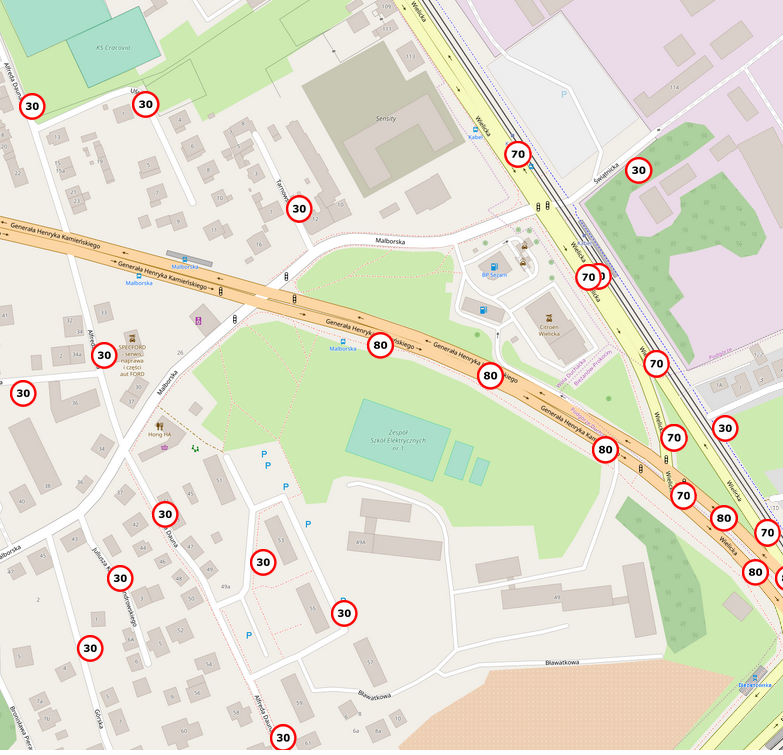
\includegraphics[width=0.7\textwidth]{typeOfRoad}
\end{figure}
\newpage
\section{Płynna zmiana prędkości pojazdów}


\newpage
\section{Historia wypadków}


\newpage
\section{Zakręty}


\section{Umiejscowienie znaków na drodze}
\label{sec:speedLimitLocalization}
Znaki drogowe ograniczenia prędkości są ustawione według następujących kryteriów:
\begin{itemize}
\item na początku każdej drogi
\item przed nieoznakowanymi przejściami dla pieszych
\item przed wjazdem do obszaru, w pobliżu którego znajdują się szkoły, place zabaw, duże sklepy handlowe i miejsca kultów religijnych
\item przed zakrętami
\item między znakami ograniczenia prędkości, dla których występują duże różnice prędkości
\end{itemize}


